%!TeX root = 5-diffusion.tex
\documentclass[main]{subfiles}

\begin{document}

\chapter{Xenon and krypton transport properties}
\vspace*{-1\baselineskip}


In separation processes, diffusion can either be the main performance metric or a neglected secondary parameter. There are actually two different use cases for separation using nanoporous materials: the adsorption-based separation that is mainly a thermodynamic process and the nanoporous separation membranes that relies on the kinetic properties. In a membrane-based process, the gas is sieved through a membrane material that blocks some molecules (e.g. Xe) and let other molecules (e.g.) diffuse freely. The performance of the separation is measured with the ratio of the diffusion coefficients instead of the thermodynamic selectivity we defined in chapter 2. The process of interest is, however, the adsorption-based separation performed industrially by pressure and/or temperature swing adsorption, and even if the thermodynamic selectivity is the main performance metric, the kinetic performances can improve our understanding of the adsorption process. For instance, in breakthrough experiments (a lab equivalent of a pressure swing adsorption) used to characterize the comparative adsorption performances of a gas mixture, the shape of the curve can be explained by diffusion processes. The goal of this chapter is to explore this often neglected diffusion parameter in an adsorption-based Xe/Kr separation process.

\begin{figure}[ht]
  \centering
    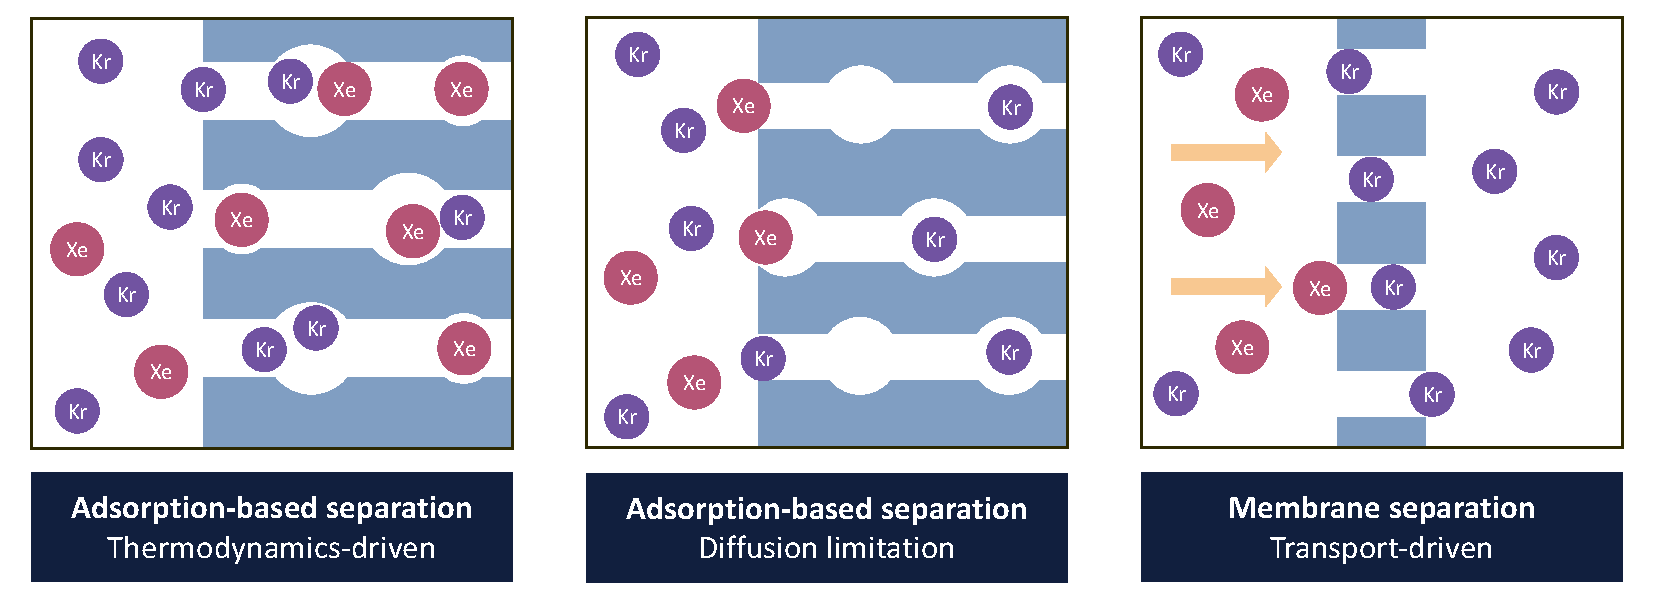
\includegraphics[width=0.95\textwidth]{figures/5-diffusion/Diffusion.pdf}
    \caption{Illustration of the comparative role of the thermodynamic and transport properties for Xe/Kr separation in nanoporous materials. From the transport dominated process of membrane separation to the thermodynamically equilibrated separation processes in the nanopores, different more nuanced cases could emerge where the diffusion imposes kinetic limitations. }
    \label{fgr:intro_diffusion}
\end{figure}

\section{Modeling Diffusion}

% From the macroscopic brownian motion modeled by the
% Fick's law
Since the pollen motion observations of the botannist Brown in 1826, scientists have observed and studied the seemingly erratic movement of particles in a static bulk medium. Later, Fick proposed a macroscopic model of this so-called brownian motion by introduced the coefficient $D$ of a diffusion equation~\ref{eq:fick} (1D) based on experimental measures of the concentration $\phi$.\autocite{Fick_1855} According to this law, at the macroscopic level, the particles tend to go move from the most concentrated area of the bulk to the less concentrated one. 

\begin{equation}\label{eq:fick}
  \frac{\partial \phi}{\partial t} = D_x \frac{\partial^2 \phi}{{\partial x}^2}
\end{equation}

To better understand the brownian motion of suspended particles on a liquid Einstein derived a microscopic model of the diffusion motion based on the molecular-kinetic theory of heat on the miraculous year of 1905.\autocite{einstein1905motion} To determine the so-called self-diffusion coefficient, he followed the motion of a particle assumed independent from other particles and time steps large enough to consider mutually independent two consecutive motions.  By using the particle distribution of N independent diffusing particle, he redefined the diffusion coefficient as a function of the mean square displacement of a particle. In a tridimensional space, we have the following Einstein relation:
\begin{equation}
  \langle r(t)^2 \rangle = 6Dt
\end{equation}
where $r(t)$ is the displacement of a particle from the time $0$ to $t$. The brackets represent the average over all independent trajectories (different particles and different time origins). This equation can be generalized to the diffusion of an adsorbate in the adsorbed phase, which describes how easy it is for a particle to move inside a nanoporous material. A low diffusion coefficient means a limited access to the pores of the structure as illustrated on Figure~\ref{fgr:intro_diffusion}.

Using molecular simulations of the adsorbate displacements, we will try to model the diffusion coefficient of xenon and krypton inside a nanoporous material. Although other approaches like the Green-Kubo equation exist the relatively less complex Einstein law is prefered for self-diffusion calculations, as shown by the following comparative study~\cite{Maginn_2020}. In this section, we will focus on the different simulation techniques that can be used to evaluate the diffusion in high-throughput screenings. We will try to present different ways of accessing the mean square displacement of a diffusing particles, by beginning from the most straight-forward molecular dynamics to faster methodologies more suitable in screenings such as machine learned surrogate models and kinetic monte carlo simulations.


\subsection{Molecular dynamics}

Molecular dynamics are used to simulate the motion of molecules in a given system. It is usually used to calculate thermodynamic averagings.\todo{give some examples} Here, we are going to focus on the calculation of diffusion coefficients of monoatomic molecules.

\subsubsection{Simulation details}

Molecular dynamics (MD) aims at describing the motion of particles subjected to the forces of the surrounding particles. It can therefore be seen as a complex integration of the Newton's law of motion. A particle $i$ of position $\mathbf{r}_i$ and mass $m_i$ subjected to a force $\mathbf{F}_i$ resulting of the cumulated interactions with its surrounding is accelerated according to this equation:
\begin{equation}\label{eq:newton}
  m_i\frac{\dd^2 \mathbf{r}_i}{{\dd t}^2} = \mathbf{F}_i
\end{equation}

In a classical modeling, the forces are determined using the well-named forcefield that was previously introduced in the chapter 2. Back there, we only considered intermolecular interactions simply modeled by the Lennard-Jones (LJ) interaction potential between atom pairs, which is also what we will use in this section (of course, it is not the only way of defining a forcefield but just a simplification). Using the LJ potentials $U\ex{LJ}$ (defined in equation~\ref{eq:LJ}), we can derive a vectorial force $\mathbf{f}_{ij}$ between two atoms $i$ and $j$.
\begin{equation}
  \mathbf{f}_{ij} = - \left.\dfrac{\dd U\ex{LJ}_{ij}}{\dd r}\right|_{r=r_{ij}} \frac{\mathbf{r}_{ij}}{r_{ij}} = 24\epsilon_{ij}  \left(2\left(\dfrac{\sigma_{ij}}{r_{ij}}\right)^{12} - \left(\dfrac{\sigma_{ij}}{r_{ij}}\right)^{6}\right) \frac{\mathbf{r}_{ij}}{r_{ij}^2}
\end{equation}
where $\epsilon_{ij}$ and $\sigma_{ij}$ are the LJ parameters of the pair of atoms $ij$. And the resulting force is simply the sum of the forces $\mathbf{F}_i=\sum_{j}\mathbf{f}_{ij}$ exerted by the surrounding atoms $j$. To reduce the computation time required, molecular simulations only consider the atoms within a given cutoff radius. 

Now that we defined the force $\mathbf{F}_i$, we can put a molecule in motion by integrating the equation~\ref{eq:newton} from a time $t$ to a time $t+\delta t$. There are different methods to integrate equation of motion such as the Euler or velocity-Verlet scheme presented in the book of Frenkel et al.\autocite{frenkel2001md} Here, we will focus on the \emph{leap frop} integration implemented in the Raspa2\autocite{dubbeldam2016} software that we used for our simulations. The position $\mathbf{r}_i$ and the velocity $\dot{\mathbf{r}}_i$ are between each time step $\delta t$ using the following equations:
\begin{equation}
  \begin{split}
    \dot{\mathbf{r}}_i\left(t+\tfrac{1}{2}\delta t\right) & = \dot{\mathbf{r}}_i\left(t-\tfrac{1}{2}\delta t\right) + \tfrac{1}{m_i}\mathbf{f}_i \\
    \mathbf{r}_i\left(t+\delta t\right) & = \mathbf{r}_i\left(t\right) + \dot{\mathbf{r}}_i\left(t+\tfrac{1}{2}\delta t\right)\delta t
  \end{split}
\end{equation}
From the initial conditions $(\mathbf{r}_i(0),\dot{\mathbf{r}}_i(0.5\delta t))$, we can translate the center of mass of the molecule $i$ to any position $\mathbf{r}_i(t_n=n*\delta t)$. We will skip the rotation step required for polyatomic molecules since we are restricting the study on the monoatomic noble gas. The different positions $\left(t_n,\mathbf{r}_i(t_n)\right)$ constitute the trajectory of the MD simulation.


\subsubsection{Diffusivity calculation using the trajectory}

The MD trajectory can be used to generate displacement of any size $\tau$.

\todo{cite some studies/review daglar > ref chapter 1}

\subsection{Kinetic Monte Carlo}

\subsubsection{Transition state theory}


\todo{what is a transition state for diffusion?}

\subsubsection{Construction of the Markov chain}

\todo{Detect TS, and bassins.}

Fast kinetic Monte Carlo
tutrast\autocite{Mace_2019} autre étude avant aussi

\subsubsection{Generation of trajectories}

\subsection{ML modeling}


\section{Transport properties of xenon/krypton separation}

\todo{We have generated diffusion coefficients for the ... best materials}

\subsection{Why studying diffusion for xenon krypton}

% si on s'intéresse à la régénération par exemple (petit problème). barrière cinétique d'entrée et de sortie.
% courbe de percée de la publi banerjee> une partie est expliquée par la diffusion également.
\todo{kinetic KAXQIL problem}

\subsection{Structure--diffusivity relationships}

\todo{correlation with VF/SA/Selectivity/permselectivity}

\begin{figure}[ht]
  \centering
    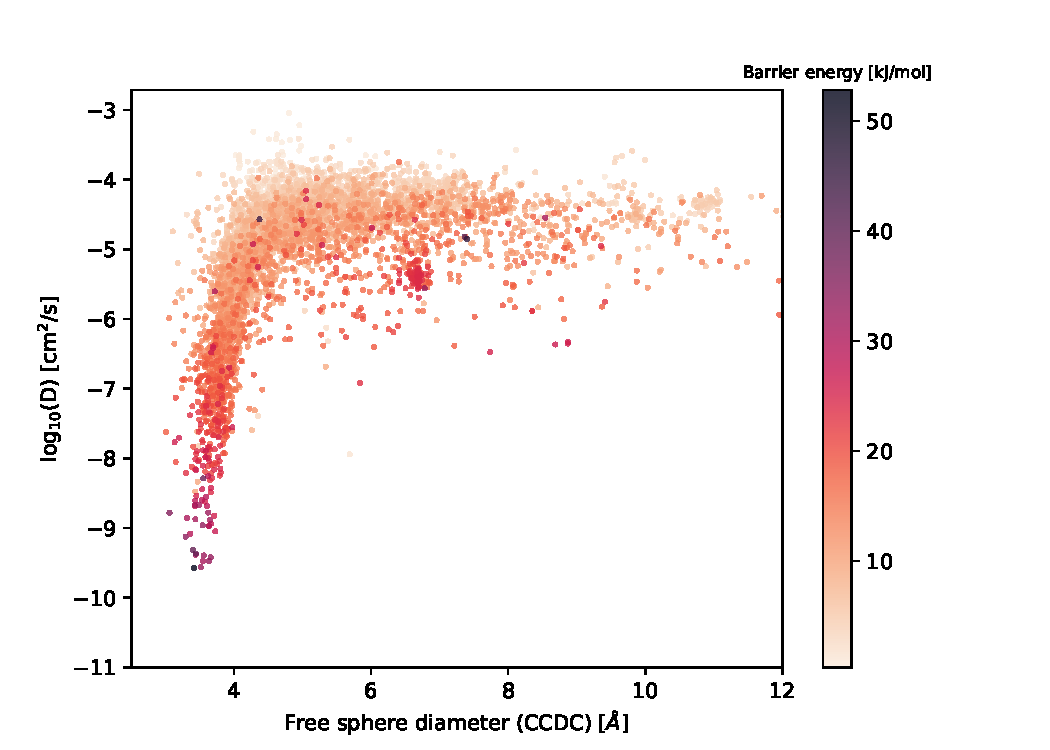
\includegraphics[width=0.48\textwidth]{figures/5-diffusion/difflog_Df-ccdc_barrier.pdf}
    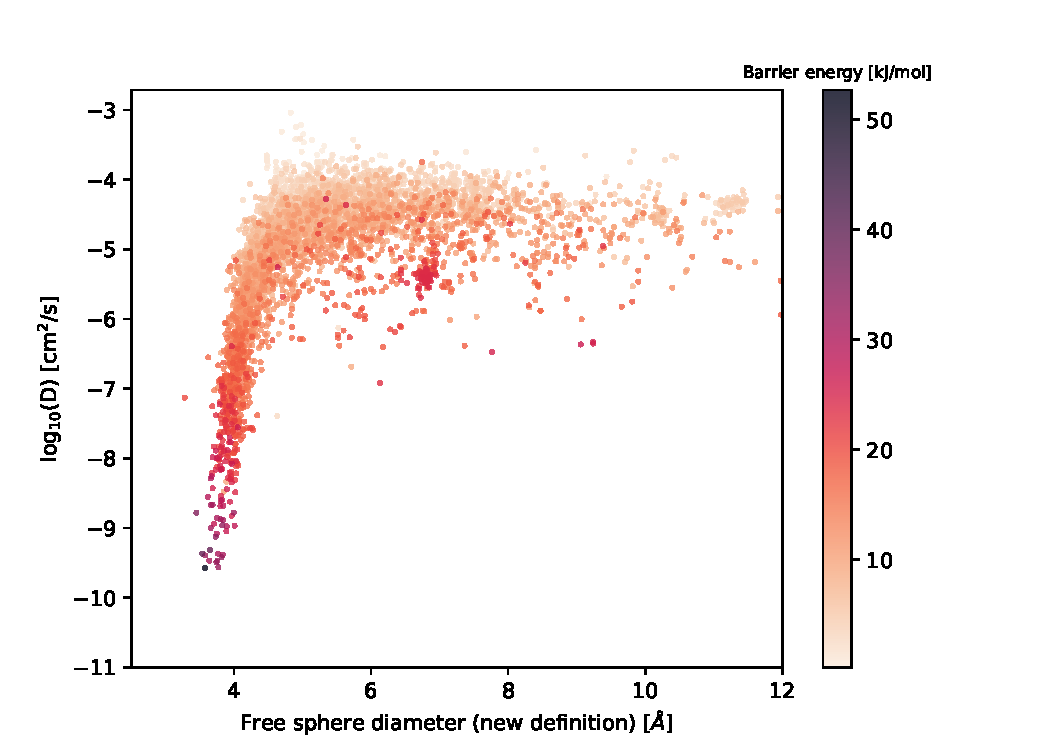
\includegraphics[width=0.48\textwidth]{figures/5-diffusion/difflog_Df-uff298K_barrier.pdf}
    \caption{\todo{correlation with PLD without labeling}}
    \label{fgr:}
\end{figure}


% Outre l'exemple très parlant de SBMOF-1, d'autres publications, dans la séparation d'hydrocarbures notamment, s'intéressent aux éventuelles blocages cinétiques grâce à des simulations de dynamique moléculaire (MD) flexible.\cite{Stanton_2022} Ils ont notamment mis en évidence que la diffusion pouvait détériorer les performances de structure présentant d'excellente performance thermodynamique (énergie d'adsorption). Cette approche est très complète, car elle allie la thermodynamique, la flexibilité et les effets de transport dans une seule étude. En revanche, elle est très coûteuse en temps de calcul et ne pourrait être appliquée qu'à une poignée de structures. Au lieu d'utiliser des champs de force flexible qui alourdissent énormément la simulation, il est possible de se tourner vers une approche en ``snapshot'' bien moins coûteuse que nous développerons dans la dernière partie de ce rapport. Dans cette partie, nous nous focaliserons uniquement sur le couplage thermodynamique/cinétique.

% Afin de recouper nos données purement structurelles et thermodynamiques avec des propriétés de transport, on a effectué un screening des coefficients de diffusion du xénon et du krypton sur les 7822 structures les plus sélectives. 
% Des trajectoires de dynamique moléculaire ont été calculées sur l'ensemble de ces structures deux fois pour chaque adsorbat à dilution infinie. Il a fallu environ une à deux journées de simulation par structure afin de déterminer leurs coefficients de diffusion. Il est à noter pour la suite que les valeurs de diffusivités sont déterminés à l'ordre de grandeur près. Autrement dit c'est l'échelle logarithmique qui est pertinent pour les comparer à d'autres grandeurs. On a pu établir une forte corrélation entre le coefficient de diffusion et la taille minimale des canaux de diffusion à l'intérieur du matériau (PLD). La figure~\ref{fgr:Diff_Df_s} met en évidence la corrélation linéaire entre le logarithme de la diffusivité et le LCD pour des canaux de taille inférieure au diamètre cinétique du xénon (\SI{4,3}{\angstrom}). Ensuite, on arrive sur un plateau, c'est-à-dire que la diffusion du xénon dans le matériau ou dans le vide sont quasiment équivalentes. Les canaux sont assez larges pour permettre la libre diffusion du xénon à l'intérieur de ces matériaux. On voit aussi que ces matériaux ont moins de chances d'être sélectifs (les points foncés sont plus rares). Cette corrélation ouvre la voie au développement de modèles statistiques pour prédire la diffusivité, ce qui a déjà été étudié par Daglar \emph{et al.} dans leur récente publication.\cite{Daglar_2022} Dans leur étude, pour l'hélium, le coefficient de corrélation entre les coefficients de diffusion prédites et calculés par MD est d'environ 0,65 pour les données de test, ce qui n'est pas très précis. Il faut donc nuancer l'approche ``machine learning'' pour la prédiction des diffusivités. Cependant, l'étude n'a pas encore été menée sur le xénon et le krypton, ce qui pourrait mériter une étude préliminaire.

\begin{figure*}[t]
\centering
  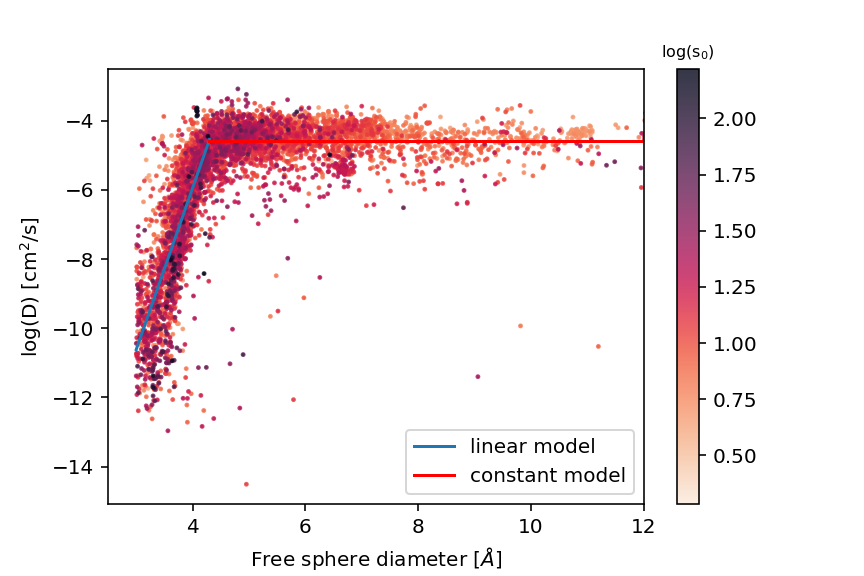
\includegraphics[width=0.8\textwidth]{figures/5-diffusion/D_log-diameter_colored_s_models+.png}
  \caption{\small{\ Logarithme du coefficient de diffusion du xénon à la limite des basses pressions en fonction du diamètre de la plus petite sphère libre dans le matériau (LCD). Les points sont colorés en fonction du logarithme de la sélectivité à basse pression $\log(s_0)$.}}
  \label{fgr:Diff_Df_s}
\end{figure*}


\subsection{Identification of interesting materials}


% En analysant les rapports des coefficients de diffusion en comparaison des sélectivités, on a pu identifier deux structures qui couplent une bonne sélectivité à un ratio de diffusivités autour de 0,5 (\emph{cf.} table~\ref{table:diff}) : les structures de code CCSD GUMDEZ et QOZDOY. Grâce à leur LCD proches du diamètre cinétique du xénon et à un PLD assez élevé pour ne pas entraver le déplacement du xénon à travers les canaux. Les coefficients de diffusion du xénon tournent autour de 7$\times$10\ex{-5} \SI{}{\square\centi\meter\per\second} ce qui est proche de la diffusion libre (de l'ordre de 10\ex{-5} \SI{}{\square\centi\meter\per\second}), ce qui confirme l'absence de blocage cinétique. 

% Une autre structure, ADOGEH (\emph{cf.} table~\ref{table:diff}), présente une diffusion 14 fois plus rapide pour le xénon que le krypton, tout en ayant une sélectivité à basse pression de 49. Ce phénomène s'explique par le fait que la structure a des canaux dans les trois directions et que pour changer de direction il faut passer par un canal plus étroit non accessible par le xénon. Ainsi le xénon, n'ayant qu'une direction de diffusion à l'intérieur du matériau, va bien plus vite que le krypton pour lequel toutes les directions s'offrent à lui. Ainsi, le krypton est plus lent à diffuser car il change de direction constamment dans le matériau contrairement au xénon. En revanche, la sélectivité baisse à 10 lorsque l'on considère un mélange de 20/80 Xe/Kr à pression ambiante au lieu de la dilution infinie. Ce matériau pourrait être utile notamment à pression partielle faible en xénon et krypton, ce qui est le cas pour notre application. Des études plus approfondies sont encore à mener, notamment en confirmant les valeurs de sélectivité par des calculs DFT plus fiable ou en étudiant la flexibilité ; mais si les résultats sont concluant ces matériaux pourraient alors être testés expérimentalement pour une éventuelle application industrielle.

\begin{table}[t]
\centering
\begin{tabular}{|l|r|r|r|r|r|r|}
\hline
  CCSD ref. code &      LCD (\SI{}{\angstrom}) &    s$_1$ &       s$_0$ &     PLD (\SI{}{\angstrom}) &     Ratio Diff. &  Coeff. de Diff. Xe \\
\hline
QOZDOY\cite{Zhang_2001} &  5,3 & 37 & 52 & 4,7 &  0.4 &               7$\times$10\ex{-5} \SI{}{\square\centi\meter\per\second} \\
GUMDEZ\cite{Yin_2014} &  5,3 & 42 & 56 & 4,8 &  0.5 &               7$\times$10\ex{-5} \SI{}{\square\centi\meter\per\second} \\
ADOGEH\cite{Peikert_2012} & 12,7 &  10 & 49 & 5,1 & 14 &               5$\times$10\ex{-5} \SI{}{\square\centi\meter\per\second} \\
\hline
\end{tabular}
\caption{\ Performances de structures identifiées par un screening prenant en compte les coefficients de diffusion. }
\label{table:diff}
\end{table}

% Les résultats d'un screening couplant thermodynamique et cinétique permettent déjà de mettre en valeur des matériaux encore inconnus de la communauté. La question du blocage cinétique est certes traitée dans certaines études,\cite{Stanton_2022} mais aucune approche systématique n'a encore été développée. Ces structures ont des sélectivités élevées mais ne sont pas les plus sélectives; elles auraient donc été écartées dans un screening standard basé uniquement sur la thermodynamique. 

% Cette approche basée sur des trajectoires de dynamique moléculaire présente toutefois ses propres défauts. En effet, la méthode est très lente (quelques jours de simulation par structure), les structures avec différents canaux non connectées posent problème car l'adsorbat ne peut diffuser que dans un seul des deux canaux. Ainsi, il faudrait dans certains cas faire plusieurs trajectoires ce qui demande encore davantage de temps de calcul. De plus, si l'on veut ajouter de la flexibilité, cette méthode ne pourrait être utilisée que sur quelques structures. C'est pourquoi, un algorithme bien plus efficace est en cours d'implémentation en C++ pour accélérer les calculs de diffusivité. Un tel algorithme est déjà conçu par le groupe de Berend Smit à l'EPFL \cite{Mace_2019}, mais le code étant sous Matlab (langage peut efficace), il est impossible de l'utiliser dans des procédures de screening. Cet algorithme détermine des sites d'adsorption et des états de transition pour passer d'un site à un autre. Puis à l'aide de simulations de Monte Carlo cinétique l'adsorbat se déplace d'un site à un autre au rythme d'une constante cinétique déterminée par l'état de transition. Cette méthode permet également d'identifier en avance les différents canaux et on assure que chacun d'entre eux sont traversés par des molécules. Par conséquent, ce nouveau code permettrait de résoudre les problèmes de temps de calcul et de fiabilité rencontrés avec la dynamique moléculaire. 

\section{Fast diffusion calculation algorithm}

\subsection{Implementation in C++}

\subsection{Preliminary results}

\subsection{Visualization tool}

\todo{Take some examples for the vizualisation with comparison to the pore size and diffusion coefficient}

\subsection{Development of a first prediction model}

\begin{figure}[ht]
  \centering
    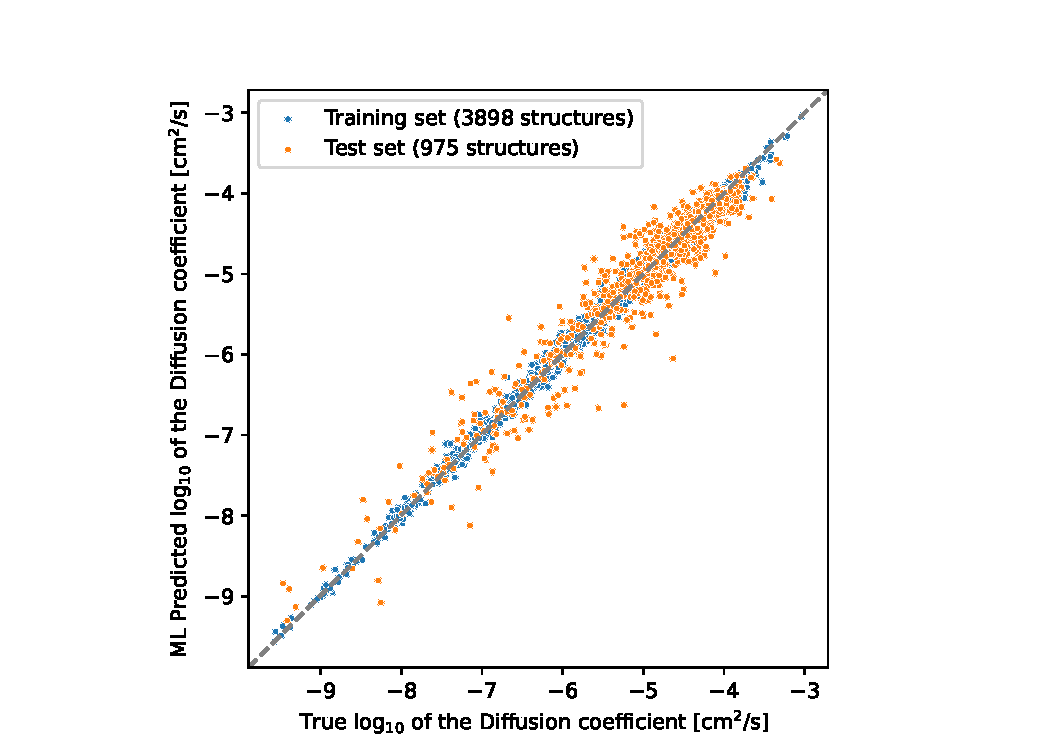
\includegraphics[width=0.48\textwidth]{figures/5-diffusion/diffusion_prediction.pdf}
    \caption{}
    \label{fgr:}
\end{figure}

\begin{figure}[ht]
  \centering
    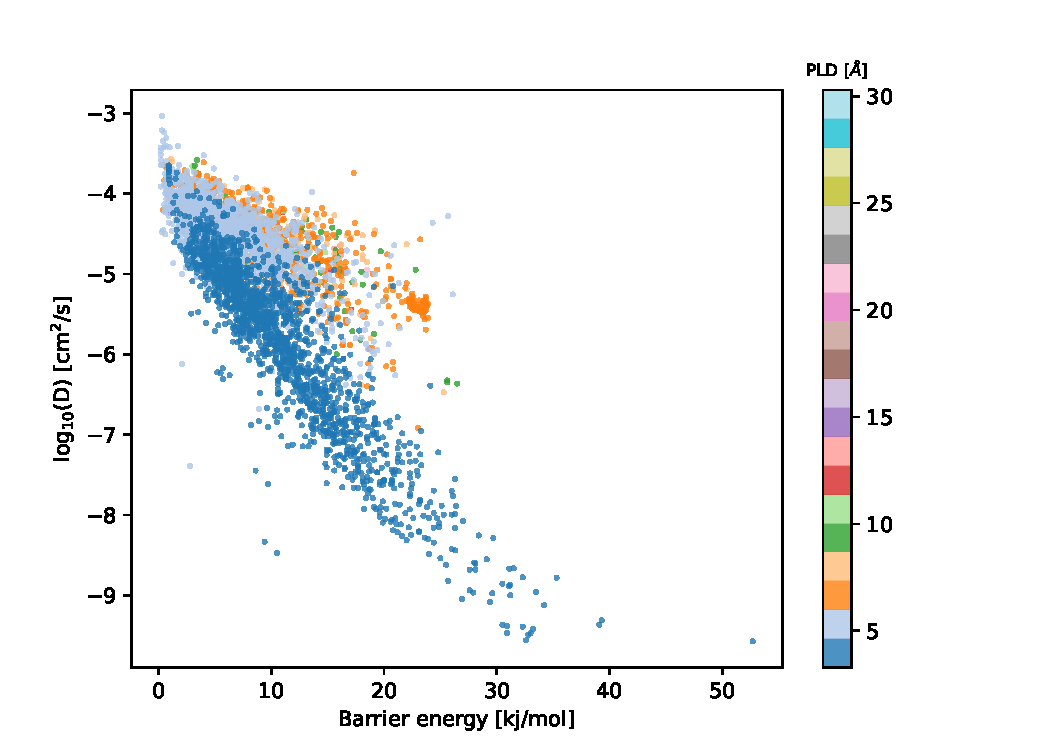
\includegraphics[width=0.48\textwidth]{figures/5-diffusion/difflog_barrier_Df_uff.pdf}
    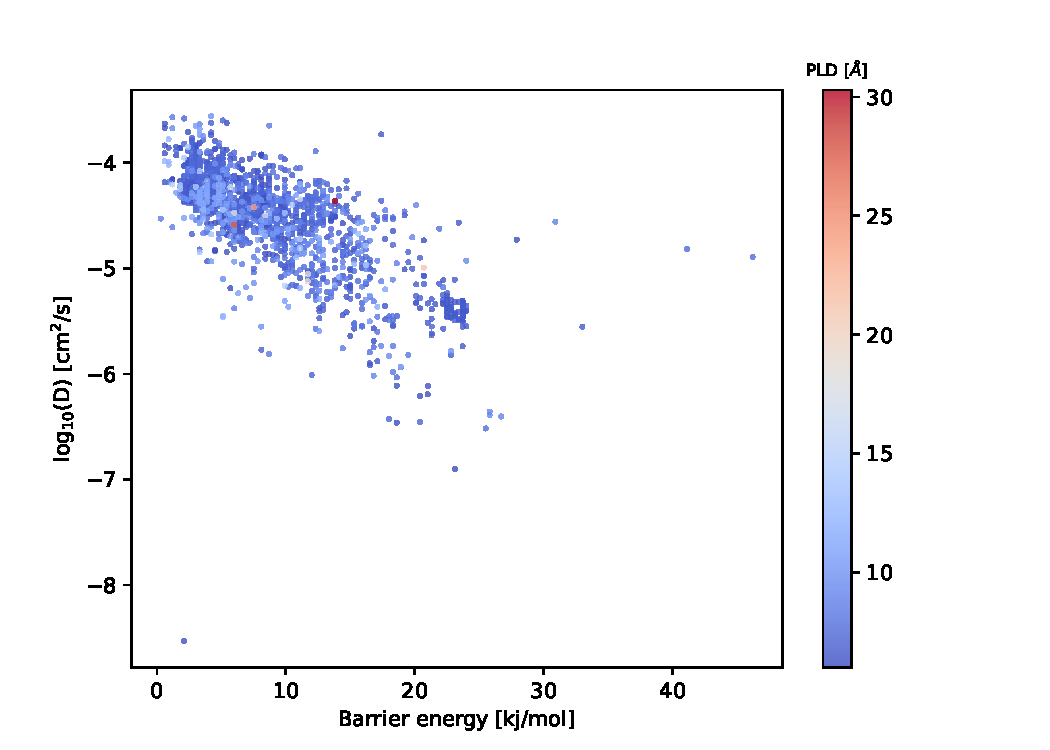
\includegraphics[width=0.48\textwidth]{figures/5-diffusion/difflog_barrier_Df_uff_2.pdf}
    \caption{}\label{fgr:}
\end{figure}

\begin{figure}[ht]
  \centering
    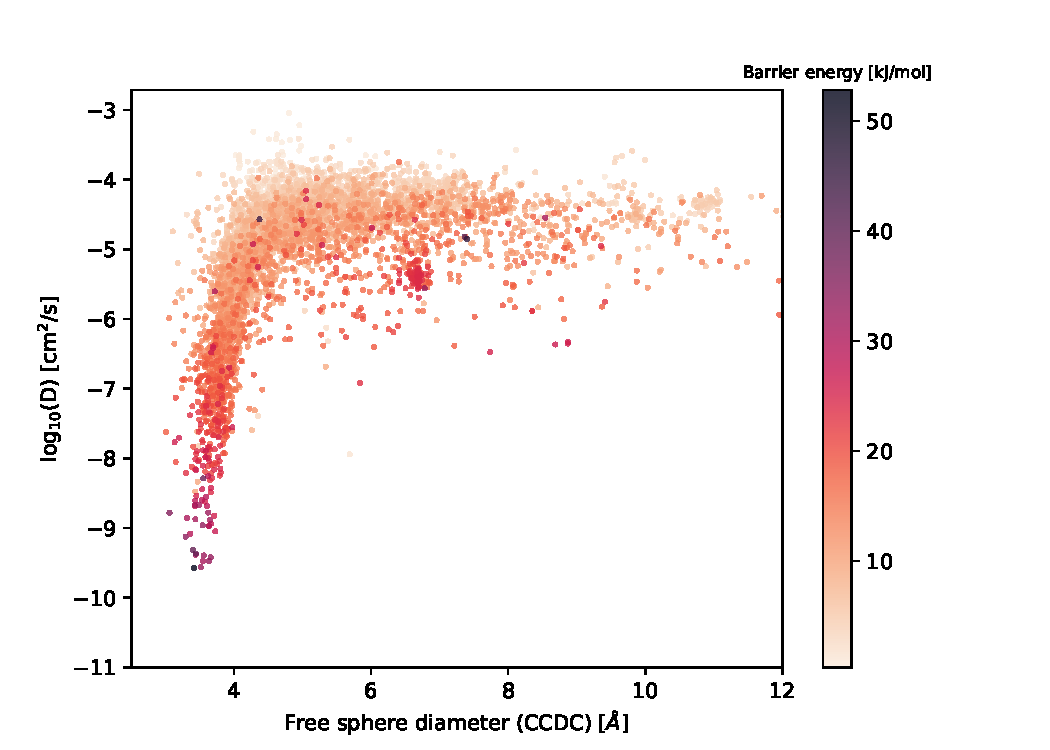
\includegraphics[width=0.48\textwidth]{figures/5-diffusion/difflog_Df-ccdc_barrier.pdf}
    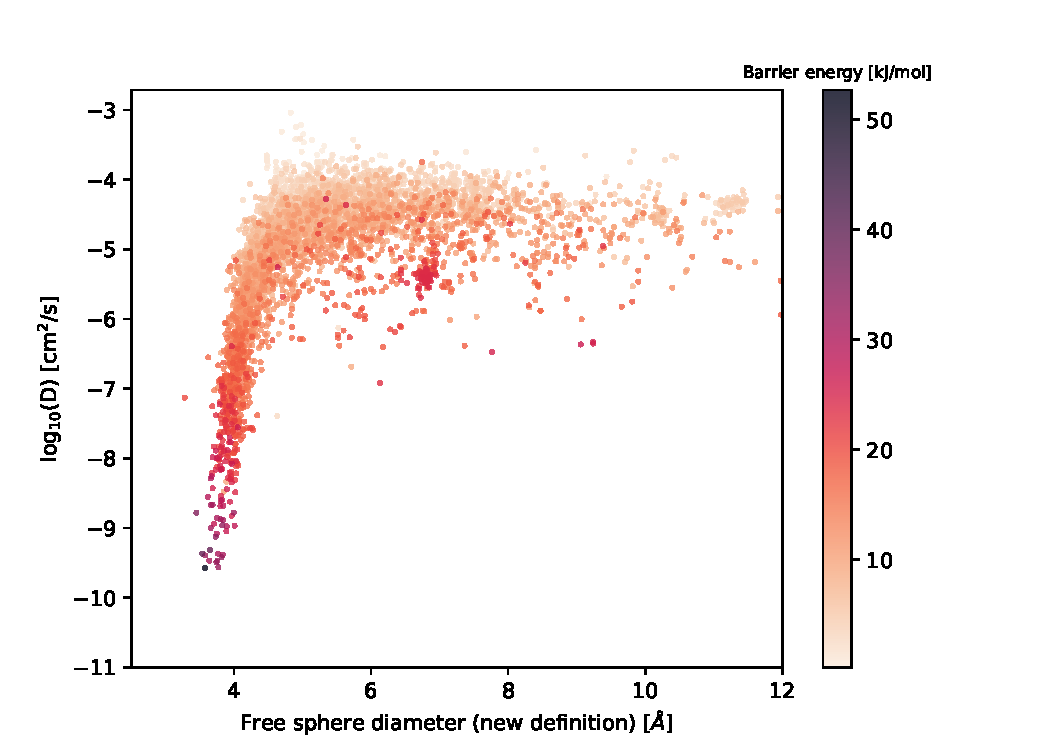
\includegraphics[width=0.48\textwidth]{figures/5-diffusion/difflog_Df-uff298K_barrier.pdf}
    \caption{}
    \label{fgr:}
\end{figure}

ML descriptors
next steps

\OnlyInSubfile{\printglobalbibliography}

\end{document}
